\documentclass[11pt,a4paper]{article}
\usepackage[utf8]{inputenc}
\usepackage[T1]{fontenc}
\usepackage{lmodern}
\usepackage[margin=1in]{geometry}
\usepackage{amsmath,amssymb,amsfonts}
\usepackage{graphicx}
\usepackage{booktabs}
\usepackage{multirow}
\usepackage{hyperref}
\usepackage[numbers,sort&compress]{natbib}
\usepackage{xcolor}
\usepackage{microtype}

\hypersetup{
  colorlinks=true,
  linkcolor=blue!60!black,
  citecolor=blue!60!black,
  urlcolor=blue!60!black
}

\title{\textbf{Calibrated Biophysical Attribution and Cross-Family Benchmarking of Pentamer DNA Shape Features in Transcription Factor Binding and Variant Specificity Shifts}}
\author{Calibrated Biophysical Attribution Consortium}
\date{November 2026}

\begin{document}
\maketitle

\begin{abstract}
Explicit structural DNA shape features---most widely derived from static pentamer lookup tables such as DNAshapeR and more recently from context-extended neural predictors such as Deep DNAshape---are routinely appended to sequence-based models to improve transcription factor (TF)--DNA binding prediction and infer shape-readout mechanisms~\cite{zhou2013nar,chiu2016bioinf,zhou2015pnas,yang2017msb,li2024natcomm,li2024nar}. However, because sequence-indexed DNA shape features are deterministic functions of local or flanking nucleotide sequence, naive ``+Shape'' performance gains over mononucleotide or dinucleotide baselines confound genuine biophysical inductive bias with unmodeled higher-order $k$-mer expansion, outer-flank receptive-field leakage, and continuous split-proxy compression in nonlinear tree learners~\cite{rube2018msb,strobl2007bmc}. Here, we establish a calibrated biophysical attribution framework combining a zero-hyperparameter conditional randomization null (\texttt{ShiftGC\_ExactCRT}) that exactly preserves reverse-complement symmetry, empirical mononucleotide--dinucleotide subspaces, cross-channel covariance, and De Bruijn shift-coboundary / Hamming-order Gram spectra~\cite{candes2018jrssb,berrett2020jrssb}, a multi-sparsity \texttt{Sparse4mer} surrogate family ($K \in \{4, 8, 12, 24, 48\}$), receptive-field flank-matched sequence baselines, and real empirical wild-type versus wild-type (WT-vs-WT) replicate negative controls. Across synthetic calibration audits ($R = 1{,}000$), external non-Fourier thermodynamic and Boltzmann simulations~\cite{santalucia1998pnas}, Exd--Hox SELEX-seq differential benchmarks~\cite{slattery2011cell,abe2015cell}, 92 disease- and structure-associated human homeodomain mutants (\texttt{GSE233827}, 30-fold leave-one-gene-out cross-validation benchmarked head-to-head with \emph{FamilyCode}~\cite{kock2024natcomm,liu2025nar}), and cross-family basic helix--loop--helix (bHLH) \texttt{Max}/\texttt{Mad1}/\texttt{cMyc} gcPBM ($N = 7{,}289$ aligned 14-bp cores) and orthogonal universal PBM (\texttt{GSE97794}, $N = 3{,}620$) cohorts~\cite{gordan2013cellrep,shen2018cels}, we obtain four unified findings. First, existing harmonic-matching nulls (\emph{Shapelizer}~\cite{rube2018msb}) suffer $4\times$ false-positive inflation ($20.0\%$ at $\alpha = 0.05$) under correlated 7-channel genomic dinucleotide nulls and up to $34.6\%$ under direct 4-mer epistasis, whereas \texttt{ShiftGC\_ExactCRT} maintains nominal control ($5.2\%$ synthetic; $4.8\%$ on multi-chamber homeodomain replicate controls; $0.0\%$ on within-array bHLH replicate controls). Second, upgrading pure-sequence baselines from dinucleotides (\texttt{Seq\_G2}) to positional 4-mers (\texttt{Seq\_Pos4mer}) or degree-3 polynomial kernels (\texttt{Poly3\_Kernel}) saturates apparent linear and kernel ``+Shape'' gains across homeodomain SELEX differentials, unseen homeodomain mutations (0/9 Holm-adjusted contrasts significant), and all 11 bHLH gcPBM/uPBM endpoints (\texttt{ShiftGC\_ExactCRT} 0/11 significant on \texttt{Seq\_Pos4mer}, $p = 0.065\text{--}0.630$). Third, in nonlinear histogram gradient-boosted decision trees (\texttt{HGBDT}), matched surrogate tables reproduce $100\%$ of apparent ``+Shape'' lifts across all 11/11 bHLH gcPBM and uPBM endpoints ($0/11$ significant at $B = 49$, $p = 0.060\text{--}0.820$), $100\%$ of the $500$/mutant homeodomain $\Delta z$ lift ($p = 0.560\text{--}0.900$), and $64\%\text{--}74\%$ of the full-dataset ($K = 2{,}000$) homeodomain specificity-orthogonalized $\Delta z_{\mathrm{spec}}$ lift under formal $\alpha = 0.05$ power ($B = 19$, $p_{\min} = 0.050$: \texttt{ShiftGC} $p = 0.050$, $p_{\mathrm{Holm}} = 0.100$; \texttt{Sparse4mer\_K12} $p = 0.150$ with $2/19$ random draws exceeding real DNAshape; N-arm $p = 0.350\text{--}0.500$; $0/6$ Holm-adjusted strata significant; excluding \texttt{HOXC10-K271E} weakens \texttt{specificity\_yes} to $p = 0.100$). Fourth, an authentic CPU comparative benchmark of pre-trained \emph{Deep DNAshape} (Layer~4, 9--10~bp receptive field) shows zero improvement over static \texttt{DNAshapeR} on 14-bp bHLH \texttt{Seq\_G2} ($-0.0012$) or \texttt{HGBDT} ($-0.0034$) and zero linear gain on \texttt{GSE233827}, while exposing receptive-field flank leakage: matching the pure-sequence flank window to Deep DNAshape's receptive field (\texttt{Pos4mer\_Flank15} on homeodomain: $+0.0276/+0.0283$; \texttt{Pos4mer\_Flank22} on bHLH single TFs) accounts for linear flank gains (\texttt{+DeepL4} on \texttt{Pos4mer\_Flank15}: $-0.0008/+0.0006$), leaving modest flank-matched residuals on bHLH \texttt{Pos4mer\_Flank22} ($+0.0050$, 4/6 Holm-sig) and nonlinear \texttt{HGBDT\_Flank15/22}.
\end{abstract}

\section{Introduction}
Sequence-specific transcription factors (TFs) decode regulatory DNA through a combination of base readout---direct hydrogen bonding and hydrophobic contacts in the major and minor grooves---and shape readout, whereby local three-dimensional DNA geometry such as minor groove width (MGW), roll, propeller twist (ProT), and helical twist (HelT) modulates electrostatic focusing and conformational deformation costs~\cite{rohs2009nature,rohs2010arb,stormo2000bioinf,lambert2018cell,afek2020nature}. Classic structural and biochemical studies established that homeodomain proteins such as \emph{Drosophila} Scr recognize narrow, electronegative minor grooves via conserved N-terminal arm arginines (Arg3 and Arg5) when complexed with Extradenticle (Exd)~\cite{joshi2007cell,slattery2011cell,abe2015cell,kribelbauer2019annrev}, while basic helix--loop--helix (bHLH) paralogs (\texttt{Max}, \texttt{Mad1}, \texttt{cMyc}) discriminate shared \texttt{CANNTG} E-box cores via flanking DNA sequence and structural properties~\cite{gordan2013cellrep,shen2018cels,rossi2018genome}.

To scale structural descriptors to genome-wide datasets, high-throughput lookup tables derived from all-atom Monte Carlo simulations---led by DNAshape, TFBSshape, GBshape, and DNAshapeR---map each overlapping DNA pentamer to static estimates of local helical and groove parameters and minor-groove electrostatic potential~\cite{zhou2013nar,yang2014nar,chiu2015nar,chiu2016bioinf,chiu2017nar,li2017nar,chiu2020nar}. Appending these pentamer-indexed features to quantitative binding models trained on protein binding microarrays (PBMs), genomic-context PBMs (gcPBMs), and SELEX-seq libraries~\cite{berger2006nbt,berger2008cell,noyes2008cell,badis2009science,jolma2013cell,riley2014mmb,weirauch2014cell} repeatedly produced statistically significant gains in cross-validated $R^2$ or Spearman correlation over mononucleotide (1-mer) and dinucleotide (2-mer) sequence baselines~\cite{mordelet2013bioinf,zhou2015pnas,dror2015genome,mathelier2016cels,yang2017msb,sielemann2021natcomm}.

Yet a fundamental statistical identifiability problem separates \emph{physical shape recognition} from \emph{statistical attribution of pentamer lookup tables}. Every static DNAshapeR feature is a deterministic real-valued function $f: \{A, C, G, T\}^5 \to \mathbb{R}^d$ of a 5-bp DNA word. Consequently, adding DNAshapeR features to a 1-mer (\texttt{Seq\_G1}) or 2-mer (\texttt{Seq\_G2}) model simultaneously injects two confounded effects: (i) potential biophysical inductive bias aligned with true 3D DNA mechanics, and (ii) generic higher-order sequence basis expansion (3-mer, 4-mer, and 5-mer terms) plus continuous feature compression that decision-tree learners can exploit as low-depth split proxies~\cite{rube2018msb,strobl2007bmc,friedman2001aos,ke2017lightgbm}. Rube et al.~(\emph{Shapelizer}~\cite{rube2018msb}) recognized this confound and introduced randomized pentamer tables matched on 1-mer/2-mer regression variance. However, independent single-channel harmonic construction fails to preserve cross-channel covariance across correlated 7-channel shape descriptors and breaks down under empirical genomic $k$-mer distributions and structured 4-mer epistasis.

A pivotal open question in regulatory genomics is whether explicit DNA shape features improve out-of-distribution generalization to \textbf{unseen protein mutations}---a central challenge for interpreting rare coding variants in human TFs~\cite{barrera2016science,demasi2011nar,christensen2012bioinf,chu2012genome,wetzel2022genome}. Kock et al.~\cite{kock2024natcomm} profiled 92 rare missense variants across 30 human homeodomain genes on universal PBMs (\texttt{GSE233827}) alongside multi-chamber WT experimental replicates, and Liu et al.~(\emph{FamilyCode}~\cite{liu2025nar}) showed that WT-trained recognition-code models predict position-specific affinity shifts ($\Delta\Delta\Delta G/RT$) on these same 92 alleles. Simultaneously, deep structural models (\emph{Deep DNAshape}, \emph{DeepPBS}, \emph{ProBound}, \emph{DeepBind}~\cite{li2024natcomm,li2024nar,mitra2024natmeth,rube2022nbt,alipanahi2015nbt,rastogi2018pnas}) underscore the urgency of establishing rigorous, leak-free null standards before attributing predictive improvements to explicit structural representations.

\section{Results}

\subsection{Three-Regime Calibration Audit and External Non-Fourier Biophysical Simulations}
We audited \emph{Shapelizer}~\cite{rube2018msb} against our exact zero-hyperparameter conditional randomization null (\texttt{ShiftGC\_ExactCRT}) across three synthetic regimes ($R = 1{,}000$ replicates each; Fig.~\ref{fig:fig1}a), after reproducing Rube et al.'s dinucleotide cross-$R^2$ decomposition (\texttt{MGW.5mer} dinucleotide cross-$R^2 = 0.875$). Under single-channel aligned uniform mononucleotide nulls (Regime~I) and single-channel unaligned 50-bp GC-stratified nulls (Regime~II), both \emph{Shapelizer} ($\mathrm{FPR} = 0.066, 0.042$) and \texttt{ShiftGC\_ExactCRT} ($\mathrm{FPR} = 0.064, 0.052$) remained near nominal calibration. Under realistic 7-channel correlated genomic enhancer sequences generated from a pure dinucleotide null (Regime~III), independent 7-channel \emph{Shapelizer} suffered a $4\times$ Type-I error inflation ($\mathrm{FPR} = 0.200$, 95\% CI $[0.176, 0.226]$ standardized; $0.202$ raw), whereas \texttt{ShiftGC\_ExactCRT} remained tightly calibrated at $\mathrm{FPR} = 0.052$ (95\% CI $[0.039, 0.068]$).

\begin{figure}[htbp]
  \centering
  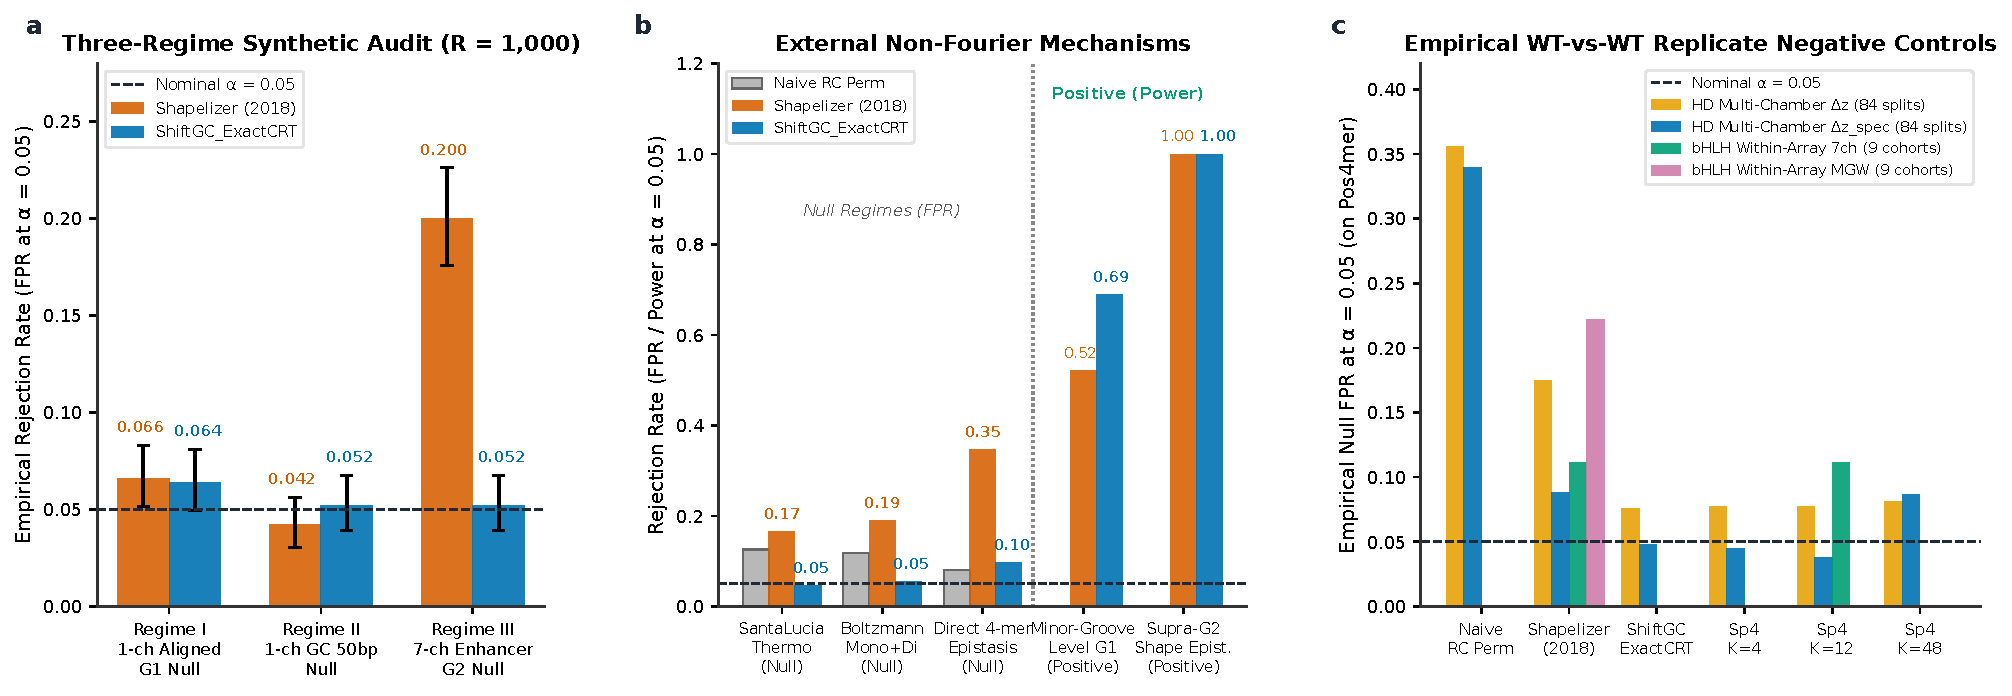
\includegraphics[width=\textwidth]{figures/fig1_calibration_and_simulations.pdf}
  \caption{\textbf{Calibration failures of naive and harmonic nulls versus \texttt{ShiftGC\_ExactCRT} across synthetic audits, external biophysical simulations, and real WT-vs-WT replicate controls.} (\textbf{a}) Three-regime synthetic audit ($R = 1{,}000$, $\alpha = 0.05$, Wilson 95\% CIs). (\textbf{b}) External non-Fourier biophysical mechanisms across three mechanistic nulls and two biophysical positive controls ($N = 500, \kappa = 0.6$). (\textbf{c}) Empirical null FPR@0.05 on real experimental WT-vs-WT replicate negative controls conditioned on \texttt{Seq\_Pos4mer} across \texttt{GSE233827} multi-chamber bipartitions (84 splits) and \texttt{GSE59845} within-array replicates (9 pairwise contrasts).}
  \label{fig:fig1}
\end{figure}

On five external non-Fourier biophysical generative models (Fig.~\ref{fig:fig1}b), both naive RC permutation ($\mathrm{FPR} = 0.126, 0.118$) and \emph{Shapelizer} ($\mathrm{FPR} = 0.166, 0.190$) severely over-rejected SantaLucia nearest-neighbor thermodynamics~\cite{santalucia1998pnas} and nonlinear Boltzmann mononucleotide+dinucleotide occupancy nulls, whereas \texttt{ShiftGC\_ExactCRT} maintained nominal error ($\mathrm{FPR} = 0.046, 0.054$). Under direct sparse 4-mer epistasis, \emph{Shapelizer} collapsed to $\mathrm{FPR} = 0.346$ while \texttt{ShiftGC\_ExactCRT} cut inflation $3.6\times$ to $0.096$. On genuine minor-groove positive controls ($N = 500, \kappa = 0.6$), \texttt{ShiftGC\_ExactCRT} delivered higher power than \emph{Shapelizer} ($0.690$ vs.\ $0.522$ at Level~G1; both $1.000$ at Level~G2).

\subsection{Empirical Replicate Negative Controls Across Multi-Chamber and Within-Array PBM Platforms}
Running our full attribution pipeline on real WT-vs-WT experimental replicates across two independent PBM platforms (Fig.~\ref{fig:fig1}c) confirmed these findings under real assay noise. On \texttt{GSE233827} multi-chamber WT-vs-WT splits (8 genes / 84 bipartitions~\cite{kock2024natcomm}) conditioned on \texttt{Seq\_Pos4mer}, naive RC permutation produced $35.6\%$ FPR on $\Delta z_{f70}$ ($34.0\%$ on $\Delta z_{\mathrm{spec}}$) and \emph{Shapelizer} remained inflated ($17.5\%$ on $\Delta z_{f70}$; $8.8\%$ on $\Delta z_{\mathrm{spec}}$), whereas \texttt{ShiftGC\_ExactCRT} achieved textbook calibration ($\mathrm{FPR} = 0.048$ on $\Delta z_{\mathrm{spec}}$; $0.076$ on $\Delta z_{f70}$), matched by \texttt{Sparse4mer} across $K \in \{4, 8, 12, 24, 48\}$ ($\mathrm{FPR} = 0.038\text{--}0.095$ on $\Delta z_{\mathrm{spec}}$). On \texttt{GSE59845} within-array technical replicates~\cite{gordan2013cellrep} (9 pairwise contrasts of rank $\le 6$ because $(r_1-r_2)+(r_2-r_3)=(r_1-r_3)$ on a single fixed sequence/table pair, reported descriptively rather than via formal i.i.d.\ KS $p$-values), \texttt{ShiftGC\_ExactCRT} yielded $\mathrm{FPR@0.05} = 0.000$ (0/9, $\mathrm{median}\ p = 0.585$) on \texttt{Seq\_Pos4mer/7ch} and $0.111$ (1/9, $\mathrm{median}\ p = 0.480$) on \texttt{Seq\_G2/7ch}, while single-channel \texttt{MGW} exhibited right-skewed conservatism ($\mathrm{median}\ p = 0.735\text{--}0.975$, $\mathrm{FPR} = 0.000$) versus $0.222$ (2/9) FPR for \emph{Shapelizer}.

\subsection{Homeodomain SELEX-seq Differentials, WT-Free Generalization, and Label-Budget Saturation}
On \texttt{GSE65073} Exd--Hox SELEX-seq differentials~\cite{slattery2011cell,abe2015cell} (Fig.~\ref{fig:fig2}), isolating the \texttt{Scr R5A--R3A} 3-way core-10 specificity shift ($N_{\mathrm{dev}} = 4{,}676, N_{\mathrm{held}} = 3{,}098$) revealed complete pure-sequence saturation: adding 7-channel DNAshape yielded $+0.0011$ on \texttt{Seq\_G2} ($0.7476 \to 0.7487$), $-0.0003$ on \texttt{Pos4mer\_N5N6} ($0.7783 \to 0.7780$), $-0.0072$ on \texttt{HGBDT} ($0.8964 \to 0.8892$), and $-0.0016$ on \texttt{Degree-3 Polynomial Kernel Ridge} ($0.9136 \to 0.9120$). This replicated on the WT-free 2-way \texttt{Scr} cohort ($N_{\mathrm{held}} = 4{,}799$, $0.9222 \to 0.9220$), across three \texttt{Antp} differentials, on unseen \texttt{Pocket6} splits (\texttt{HGBDT}: $0.7382 \to 0.7428, +0.0046, p_{\mathrm{boot}} = 0.513$), on unseen \texttt{Spacer2} splits (\texttt{HGBDT}: $0.6733 \to 0.5268, -0.1466$), and across the entire $N \in [25, 4{,}676]$ label-budget curve (Fig.~\ref{fig:fig2}c).

\begin{figure}[htbp]
  \centering
  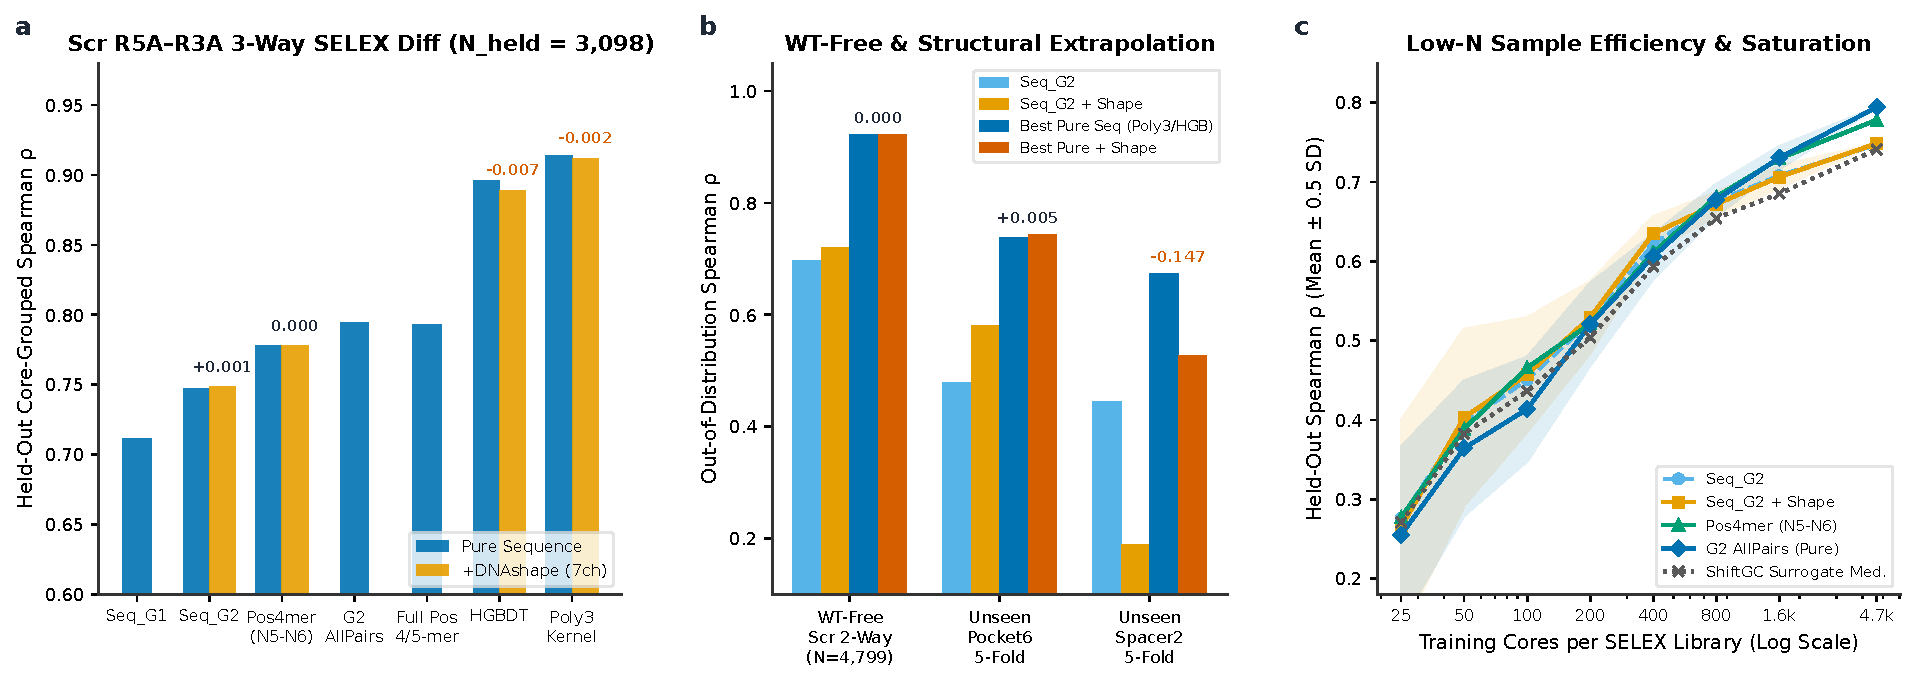
\includegraphics[width=\textwidth]{figures/fig2_selex_and_label_efficiency.pdf}
  \caption{\textbf{Pure-sequence saturation and structural extrapolation on Exd--Hox SELEX-seq mutant differentials.} (\textbf{a}) Held-out core-grouped Spearman $\rho$ ($N_{\mathrm{held}} = 3{,}098$) on 3-way \texttt{Scr R5A--R3A}. (\textbf{b}) WT-free 2-way differential ($N_{\mathrm{held}} = 4{,}799$) and 5-fold structural out-of-distribution extrapolation across unseen \texttt{Pocket6} and \texttt{Spacer2} splits. (\textbf{c}) Low-$N$ label-budget learning curves ($N = 25$ to $4{,}676$).}
  \label{fig:fig2}
\end{figure}

\subsection{Unseen Homeodomain Mutant Specificity Shifts on \texttt{GSE233827} and Matched \emph{FamilyCode} Benchmarking}
On \texttt{GSE233827} (92 missense mutants across 30 human homeodomain genes~\cite{kock2024natcomm}; Fig.~\ref{fig:fig3}), we reproduced \emph{FamilyCode}~\cite{liu2025nar} on its native $\Delta\Delta\Delta G/RT$ endpoint ($\mathrm{mean}\ R^2 = 0.3280$, $\mathrm{median}\ R^2 = 0.3261$, 73/92 alleles with $R^2 > 0$, $\max \mathrm{AUC} = 0.7126$, Kock overlap hypergeometric $p = 0.0024$; noting two pre-existing \texttt{pred\_confidence} NaNs in \texttt{ALX3-N203Q/S} at invariant \texttt{N51}). Because \texttt{GSE233827} was evaluated in the original \emph{FamilyCode} study, all comparisons are framed strictly as a matched head-to-head benchmark under explicit supervision regimes.

Across every linear Ridge interaction model with identical physical 12-bp flanks (zero \texttt{N}-padding for \texttt{N1}--\texttt{N2}), explicit DNAshape failed to improve out-of-gene generalization (Fig.~\ref{fig:fig3}a--b): Regime~A WT-only \texttt{Seq\_G1+Shape} trailed pure \texttt{Seq\_G1} ($0.0434$ vs.\ $0.0507, \Delta = -0.0073, p = 0.112$); Regime~B 30-fold LOGO linear models yielded negative deltas on $\Delta z_{f70}$ (\texttt{Seq\_G1}: $-0.0055$; \texttt{Seq\_G2}: $-0.0043$; \texttt{Pos4mer}: $-0.0070$, all $p \ge 0.194$) and on $\Delta z_{\mathrm{spec}}$ (\texttt{Pos4mer}: $-0.0073$); and Kock 8-mer \texttt{T3D4} summaries yielded $\Delta = -0.0001$ ($p = 0.906$) and $+0.0002$ ($p = 0.595$) on \texttt{Pos4mer\_T3D4}. Full-$K=2{,}000$ nonlinear \texttt{HGBDT} (\texttt{HGBDT\_Mut\_x\_Seq} $= 0.1006$ on $\Delta z_{f70}$ and $0.1268$ on $\Delta z_{\mathrm{spec}}$, the strongest pure-sequence model) exhibited nominal raw lifts in LOGO ($\Delta z_{f70}$: $+0.0171, p = 0.0212$; $\Delta z_{\mathrm{spec}}$: $+0.0162, p = 0.0164$) and non-significant lift in LOMO ($+0.0154, p = 0.110$). Across the 9 headline cross-regime contrasts (Fig.~\ref{fig:fig3}b), 0/9 survived Holm--Bonferroni adjustment ($p_{\mathrm{Holm}} = 0.148\text{--}1.000$).

\begin{figure}[htbp]
  \centering
  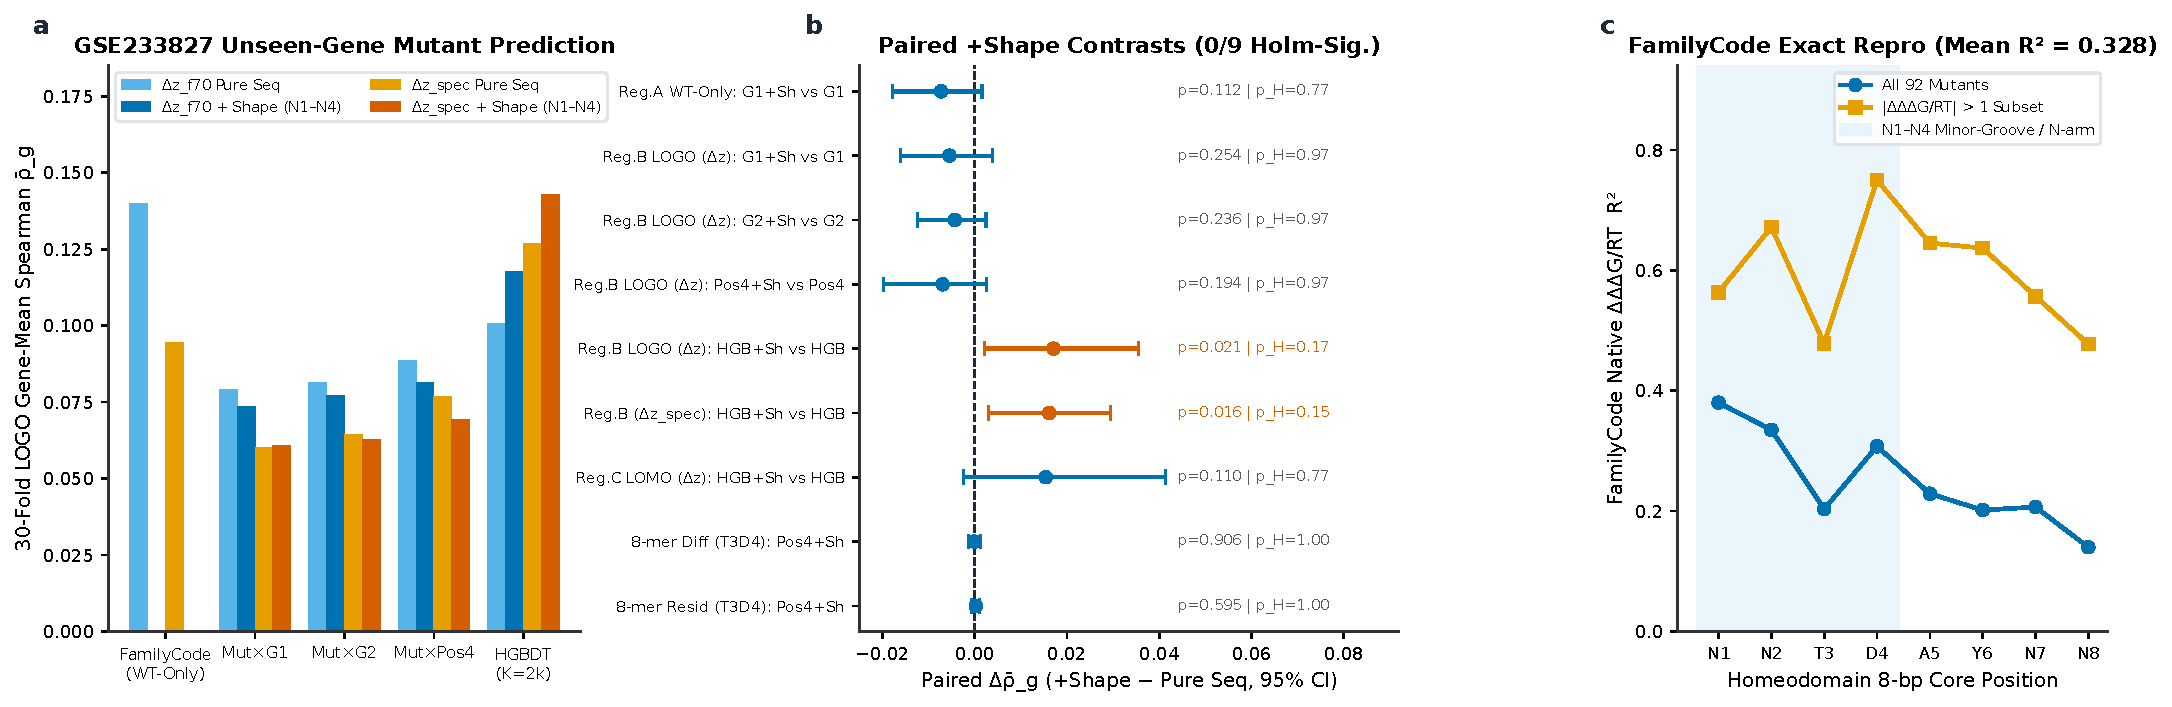
\includegraphics[width=\textwidth]{figures/fig3_gse233827_hd_mutants_and_familycode.pdf}
  \caption{\textbf{Predicting binding specificity shifts of unseen human homeodomain mutants (\texttt{GSE233827}, 92 alleles across 30 genes).} (\textbf{a}) 30-fold LOGO gene-mean Spearman $\bar{\rho}_g$ across $\Delta z_{f70}$ and $\Delta z_{\mathrm{spec}}$. (\textbf{b}) Paired gene-clustered 95\% CI forest plot across 9 headline contrasts (0/9 Holm-significant). (\textbf{c}) Exact \emph{FamilyCode} native per-position $\Delta\Delta\Delta G/RT$ $R^2$ profile across \texttt{N1}--\texttt{N8}.}
  \label{fig:fig3}
\end{figure}

\subsection{Decomposing Nonlinear \texttt{HGBDT} Lifts via Matched Surrogates and \texttt{HOXC10-K271E} Sensitivity}
Using our \texttt{High-Resolution HGBDT Matched Surrogate Evaluator} with locked hyperparameters and exact startup parity ($0.00\times 10^0$ in Exp~1a and Exp~1b $B=19$ across all 338 reused draw 0--8 scalars; $\le 1.07\times 10^{-8}$ in the Exp~1b $\Delta z_{f70}$ bridge), we decomposed nonlinear \texttt{HGBDT} lifts across Exp~1a ($500$/mut, $B = 49$) and full-$K = 2{,}000$ Exp~1b ($183{,}982$ rows: $B = 9$ effect-size bridge on $\Delta z_{f70}$ and formally powered $B = 19$ extension with $p_{\min} = 0.050$ achieving formal $\alpha = 0.05$ power on $\Delta z_{\mathrm{spec}}$; Fig.~\ref{fig:fig4}; Table~\ref{tab:hgbdt}).

\begin{figure}[htbp]
  \centering
  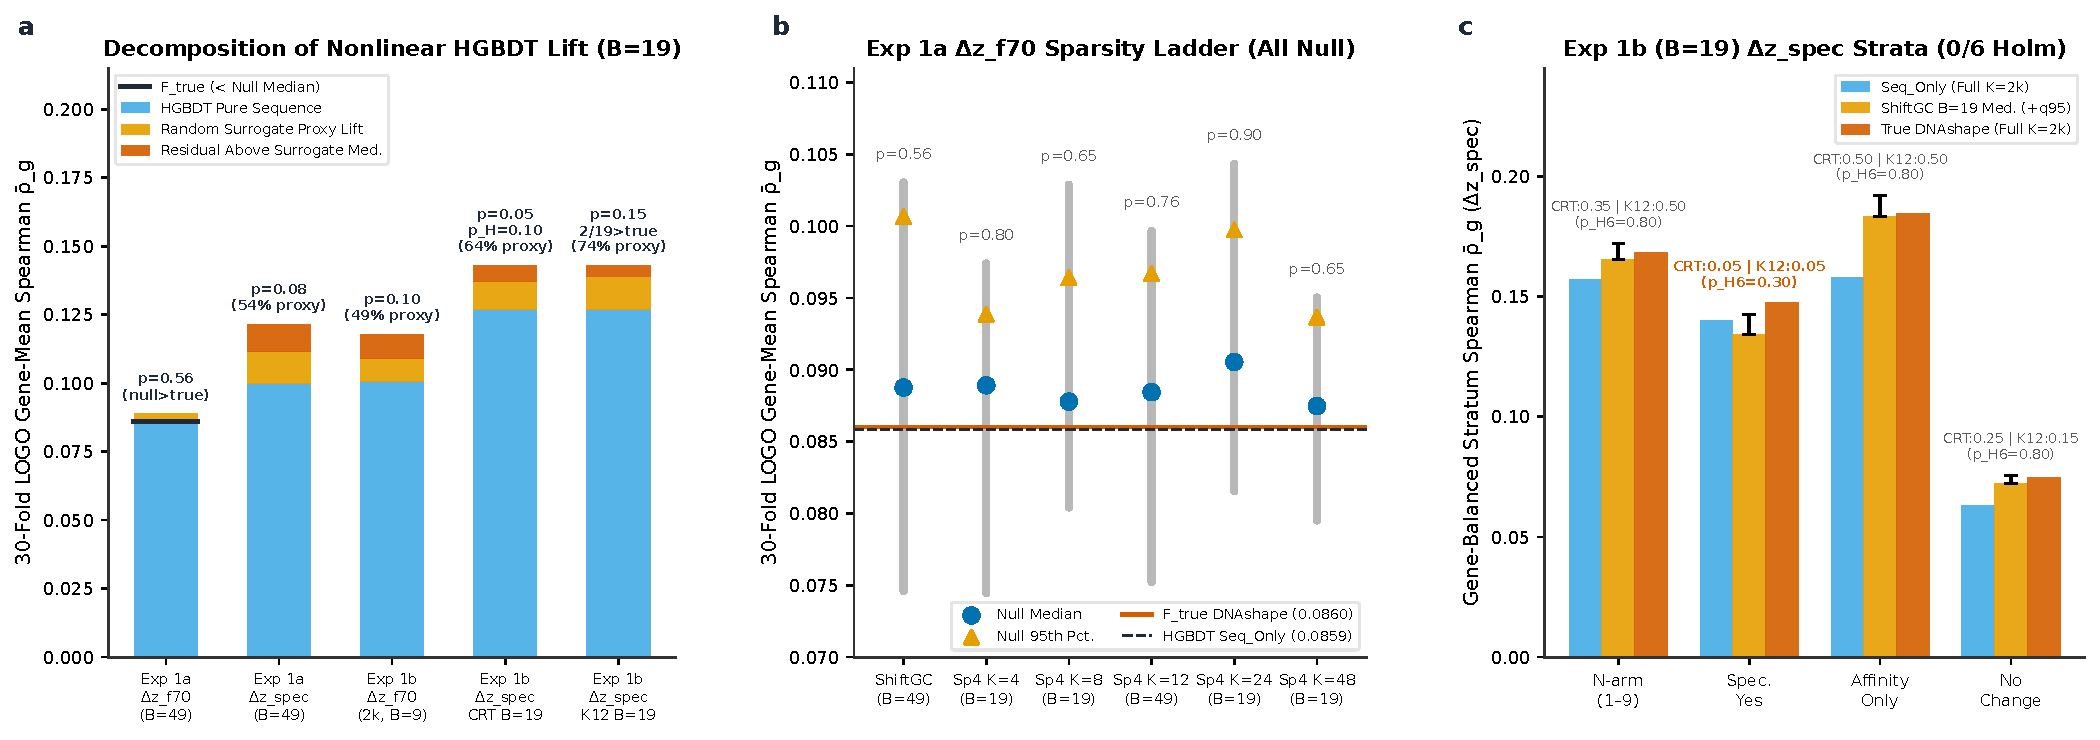
\includegraphics[width=\textwidth]{figures/fig4_hgbdt_surrogate_decomposition.pdf}
  \caption{\textbf{Matched-surrogate decomposition of nonlinear \texttt{HGBDT + DNAshape} lifts on \texttt{GSE233827}.} (\textbf{a}) Stacked decomposition of 30-fold LOGO $\bar{\rho}_g$ into pure-sequence baseline, random surrogate proxy lift (64\% \texttt{ShiftGC}, $p = 0.050$, $p_{\mathrm{Holm}} = 0.100$; 74\% \texttt{Sparse4mer\_K12}, $p = 0.150$, 2/19 draws exceeding real DNAshape at full $K=2{,}000$, $B=19$), and residual above the surrogate median. (\textbf{b}) Exp~1a $\Delta z_{f70}$ sparsity ladder ($K \in \{4,8,12,24,48\}$ and \texttt{ShiftGC}): every random surrogate median exceeds real DNAshape ($p = 0.56\text{--}0.90$). (\textbf{c}) Full-$K=2{,}000$ Exp~1b ($B = 19$) gene-balanced biological stratum breakdown on $\Delta z_{\mathrm{spec}}$ showing 0/6 Holm-significant strata (N-arm $p = 0.35\text{--}0.50$, $p_{\mathrm{H6}} = 0.80\text{--}1.00$; \texttt{specificity\_yes} raw $p = 0.05$, $p_{\mathrm{H6}} = 0.30$).}
  \label{fig:fig4}
\end{figure}

On primary $\Delta z_{f70}$, every random surrogate median ($0.0875\text{--}0.0905$) outperformed real DNAshape ($0.0860$) in Exp~1a ($p_{\mathrm{gm}} = 0.560\text{--}0.900$ across all 6 families), and random tables reproduced $49\%\text{--}54\%$ of the full-$K=2{,}000$ Exp~1b lift (with a random \texttt{Sparse4mer\_K12} draw reaching $0.1186 > 0.1177$, $p_{\mathrm{gm}} = 0.200$). On full-$K=2{,}000$ $\Delta z_{\mathrm{spec}}$ under formal $\alpha = 0.05$ power ($B = 19$, \texttt{Seq\_Only} $\bar{\rho}_g = 0.1268$ / MW $0.1259$; \texttt{F\_true} $0.1429$ / $0.1392$; lift $+0.0162$ / $+0.0133$), random tables reproduced $64\%$ of the lift under \texttt{ShiftGC} (GB median $0.1371$, $[0.1317, 0.1417]$, residual $+0.0058$, $p_{\mathrm{mc}} = 0.050$, $p_{\mathrm{Holm,2fam}} = 0.100$, $p_{\mathrm{Holm,7strata}} = 0.350$; MW median $0.1319$, $p_{\mathrm{mc}} = 0.100$) and $74\%$ under \texttt{Sparse4mer\_K12} (GB median $0.1388$, $[0.1304, 0.1444]$, residual $+0.0042$, 2/19 random draws $\ge$ true, $p_{\mathrm{mc}} = 0.150$; MW median $0.1330$, $p_{\mathrm{mc}} = 0.050$, $p_{\mathrm{Holm,2fam}} = 0.100$). Whereas all-30-gene Exp~1a ($500$/mut) initially suggested N-arm/specificity enrichment driven $68\%\text{--}69\%$ by single outlier allele \texttt{HOXC10-K271E} (collapsing to null upon excluding \texttt{HOXC10}: \texttt{ShiftGC} $p = 0.180$, \texttt{K12} $p = 0.100$), full-$K=2{,}000$ Exp~1b ($B = 19$) yields 0/6 Holm-significant biological strata ($\min p_{\mathrm{H6}} = 0.300$): \texttt{N\_arm\_1\_9} is completely null (GB/MW $p_{\mathrm{mc}} = 0.350/0.500$ for \texttt{ShiftGC}, $0.500/0.450$ for \texttt{K12}), and \texttt{specificity\_yes} sits at raw GB $p_{\mathrm{mc}} = 0.050$ ($p_{\mathrm{H6}} = 0.300$; MW $p_{\mathrm{mc}} = 0.100$, $p_{\mathrm{H6}} = 0.600$), weakening further upon excluding \texttt{HOXC10-K271E} ($p_{\mathrm{mc}} = 0.100$ GB \& MW, $p_{\mathrm{H6}} = 0.600$; \texttt{N\_arm\_1\_9} $p_{\mathrm{mc}} = 0.550\text{--}0.650$).

\begin{table}[htbp]
  \centering
  \caption{Homeodomain \texttt{GSE233827} \texttt{HGBDT} matched surrogate controls (Exp~1a $B=49$ and Exp~1b full $K=2{,}000$ $B=19$ extension).}
  \label{tab:hgbdt}
  \scriptsize
  \begin{tabular}{lcccccccccc}
    \toprule
    Experiment \& Endpoint & Seq $\bar{\rho}_g$ & True $\bar{\rho}_g$ & Surrogate ($B$) & Null Med. & Proxy Lift & Resid. & $p_{\mathrm{mc}}$ (Gene) & N-arm $p$ & \texttt{spec} $p$ & \texttt{aff} $p$ \\
    \midrule
    Exp 1a (500/m) $\Delta z_{f70}$ & 0.0859 & 0.0860 & ShiftGC (49) & 0.0888 & +0.0029 & $-0.0027$ & 0.560 & 0.640 & 0.580 & 0.380 \\
    Exp 1a (500/m) $\Delta z_{f70}$ & 0.0859 & 0.0860 & Sp4\_K12 (49) & 0.0884 & +0.0026 & $-0.0024$ & 0.760 & 0.820 & 0.680 & 0.540 \\
    Exp 1a $\Delta z_{\mathrm{spec}}$ (30g) & 0.1000 & 0.1213 & ShiftGC (49) & 0.1115 & +0.0115 & +0.0097 & 0.080 & 0.040$^{\mathrm{g}}$ & 0.020$^{\mathrm{g}}$ & 0.420 \\
    Exp 1a $\Delta z_{\mathrm{spec}}$ (30g) & 0.1000 & 0.1213 & Sp4\_K12 (49) & 0.1123 & +0.0123 & +0.0090 & 0.020 & 0.020$^{\mathrm{g}}$ & 0.020$^{\mathrm{g}}$ & 0.320 \\
    Exp 1a $\Delta z_{\mathrm{spec}}$ (29g, $-$\texttt{HOXC10}) & 0.1054 & 0.1124 & ShiftGC / K12 & 0.1071 & +0.0017 & +0.0053 & 0.180 / 0.100 & 0.160$^{\mathrm{g}}$ & 0.080$^{\mathrm{g}}$ & --- \\
    Exp 1b (Full 2k) $\Delta z_{f70}^*$ & 0.1006 & 0.1177 & ShiftGC (9) & 0.1090 & +0.0084 & +0.0087 & 0.100$^*$ & 0.200 & 0.200 & 0.300 \\
    Exp 1b (Full 2k) $\Delta z_{f70}^*$ & 0.1006 & 0.1177 & Sp4\_K12 (9) & 0.1098 & +0.0093 & +0.0078 & 0.200$^*$ & 0.100 & 0.800 & 0.200 \\
    Exp 1b (Full 2k) $\Delta z_{\mathrm{spec}}$ (30g) & 0.1268 & 0.1429 & ShiftGC (19) & 0.1371 & +0.0103 (64\%) & +0.0058 & 0.050 [0.100] & 0.350$^{\mathrm{g}}$ & 0.050$^{\mathrm{g},\dagger}$ & 0.500 \\
    Exp 1b (Full 2k) $\Delta z_{\mathrm{spec}}$ (30g) & 0.1268 & 0.1429 & Sp4\_K12 (19) & 0.1388 & +0.0120 (74\%) & +0.0042 & 0.150 [0.150] & 0.500$^{\mathrm{g}}$ & 0.050$^{\mathrm{g},\dagger}$ & 0.500 \\
    Exp 1b (Full 2k) $\Delta z_{\mathrm{spec}}$ (29g, $-$\texttt{HOXC10}) & 0.1168 & 0.1338 & ShiftGC / K12 (19) & 0.1292 & +0.0124 (73\%) & +0.0046 & 0.050 / 0.100 & 0.650$^{\mathrm{g}}$ & 0.100$^{\mathrm{g},\dagger}$ & 0.500 \\
    \bottomrule
  \end{tabular}
\end{table}

\subsection{Cross-Family Generalization to bHLH Paralog Specificity Across gcPBM and Orthogonal uPBM}
Evaluating the bHLH paralog trio (\texttt{Max}, \texttt{Mad1}, \texttt{cMyc}) across \texttt{GSE59845} paired gcPBM ($N = 7{,}289$ aligned 14-bp cores, $1{,}238$ homology groups~\cite{gordan2013cellrep}) and orthogonal \texttt{GSE97794} uPBM ($N = 3{,}620$ cores, $2{,}043$ groups~\cite{shen2018cels}) reproduced every core conclusion in a second TF family (Fig.~\ref{fig:fig5}; Table~\ref{tab:bhlh}). On gcPBM, pure-sequence \texttt{Seq\_Pos4mer} beat \texttt{Seq\_G2 + Shape} on 5/6 endpoints (including all three paralog differentials by $+0.0121$ to $+0.0347$), shrank residual ``+Shape'' gains to $-0.0004\text{--}+0.0052$, and yielded 0/6 significant endpoints under \texttt{ShiftGC\_ExactCRT} ($p = 0.205\text{--}0.585, p_{\mathrm{Holm}} = 1.000$). Crucially, locked-config \texttt{HGBDT} matched surrogates ($B = 49$) collapsed \textbf{all 11/11 bHLH endpoints} across both platforms: 0/6 significant on gcPBM (\texttt{ShiftGC} $p = 0.100\text{--}0.760$, \texttt{K12} $p = 0.240\text{--}0.820$) and 0/5 significant on orthogonal uPBM (\texttt{ShiftGC} $p = 0.060\text{--}0.200$, \texttt{K12} $p = 0.080\text{--}0.240$, all $p_{\mathrm{Holm}} \ge 0.300$). On smaller uPBM ($N = 3{,}620$), \texttt{Seq\_Pos4mer} ($p = 1{,}416$) overfits relative to \texttt{Seq\_G2}, yet \texttt{ShiftGC\_ExactCRT} remained 0/5 significant on both \texttt{Seq\_G2} ($p = 0.055\text{--}0.875$) and \texttt{Seq\_Pos4mer} ($p = 0.065\text{--}0.630$).

\begin{figure}[htbp]
  \centering
  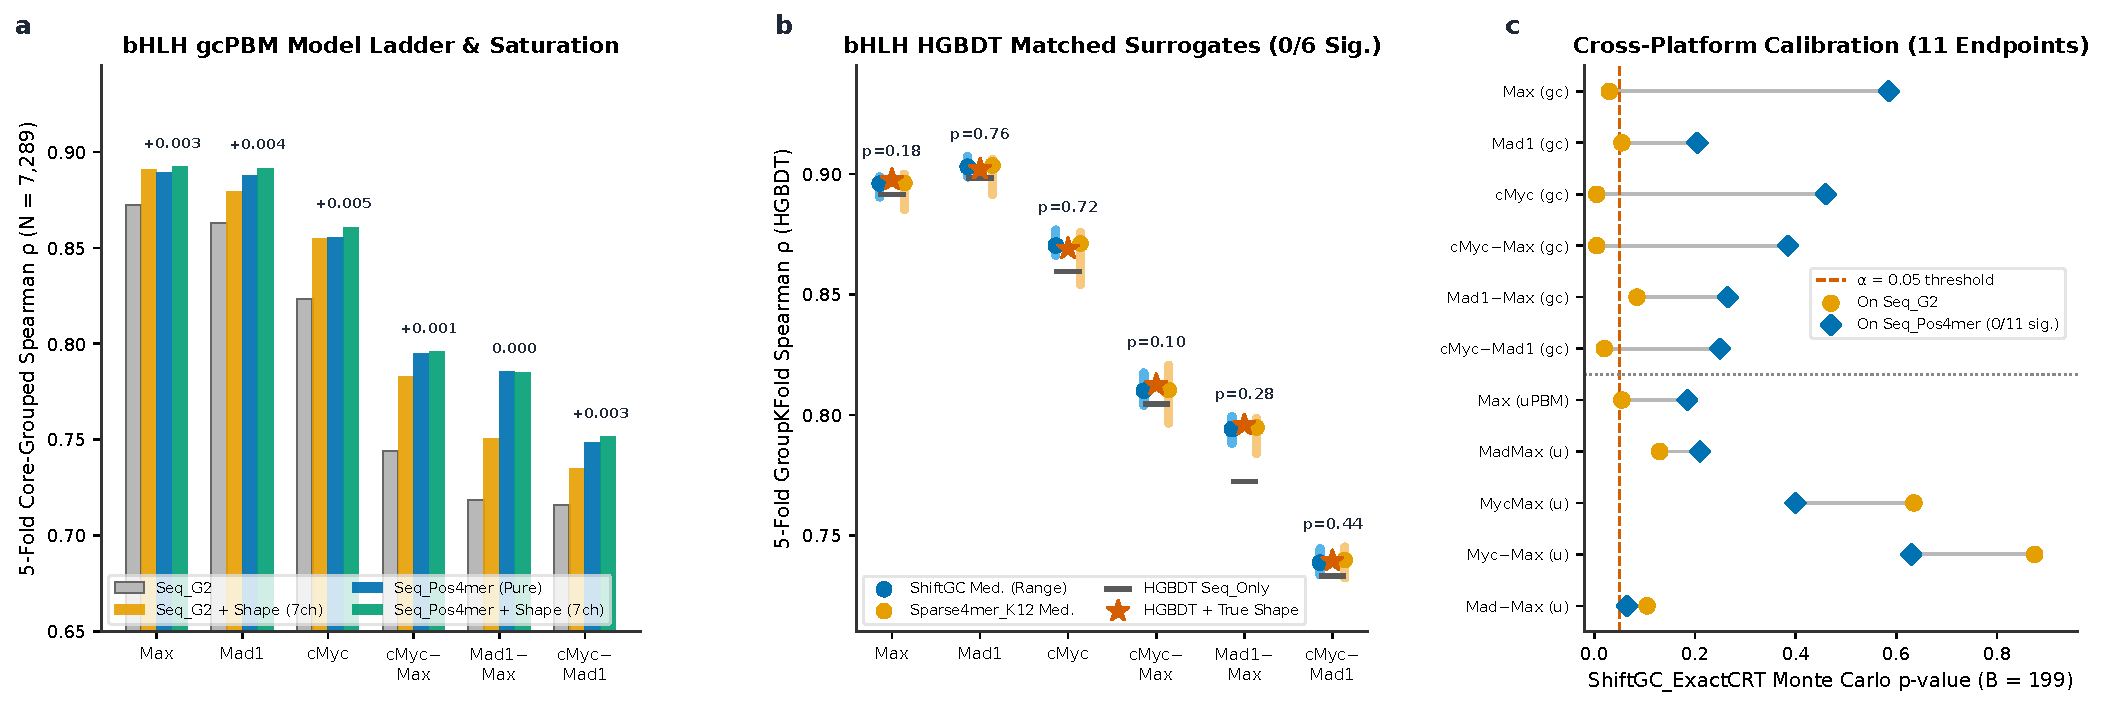
\includegraphics[width=\textwidth]{figures/fig5_bhlh_cross_family_gcpbm_upbm.pdf}
  \caption{\textbf{Cross-family bHLH (\texttt{Max}, \texttt{Mad1}, \texttt{cMyc}) model saturation and complete nonlinear surrogate collapse across gcPBM and orthogonal uPBM.} (\textbf{a}) 5-fold core-grouped Spearman $\rho$ ($N = 7{,}289$) across all 6 primary gcPBM endpoints. (\textbf{b}) Locked-config \texttt{HGBDT} matched surrogate controls ($B = 49$) across all 6 gcPBM endpoints (0/6 significant). (\textbf{c}) \texttt{ShiftGC\_ExactCRT} $p$-values ($B = 199$) on \texttt{Seq\_G2} vs.\ \texttt{Seq\_Pos4mer} across all 11 bHLH endpoints (0/11 significant on \texttt{Seq\_Pos4mer}).}
  \label{fig:fig5}
\end{figure}

\begin{table}[htbp]
  \centering
  \caption{Cross-family bHLH \texttt{gcPBM} ($N = 7{,}289$) and orthogonal \texttt{GSE97794} \texttt{uPBM} ($N = 3{,}620$) benchmark summary.}
  \label{tab:bhlh}
  \scriptsize
  \begin{tabular}{lccccccc}
    \toprule
    Endpoint & \texttt{Seq\_G2}$\to$+7ch & \texttt{Pos4mer}$\to$+7ch & \texttt{Pos4} CRT $p$ & \texttt{Poly3}$\to$+7ch & \texttt{HGB} (Locked) & \texttt{HGB} CRT $p$ & \texttt{HGB} K12 $p$ \\
    \midrule
    gcPBM \texttt{Max} & $0.8724\to 0.8910$ & $0.8893\to 0.8922$ & 0.585 & $0.8842\to 0.9048$ & $0.8914\to 0.8976$ & 0.180 & 0.240 \\
    gcPBM \texttt{Mad1} & $0.8630\to 0.8796$ & $0.8876\to 0.8916$ & 0.205 & $0.8871\to 0.9047$ & $0.8982\to 0.9021$ & 0.760 & 0.680 \\
    gcPBM \texttt{cMyc} & $0.8232\to 0.8548$ & $0.8555\to 0.8608$ & 0.460 & $0.8466\to 0.8794$ & $0.8596\to 0.8690$ & 0.720 & 0.820 \\
    gcPBM \texttt{cMyc$-$Max} & $0.7439\to 0.7830$ & $0.7951\to 0.7960$ & 0.385 & $0.7873\to 0.8090$ & $0.8045\to 0.8125$ & 0.100 & 0.260 \\
    gcPBM \texttt{Mad1$-$Max} & $0.7188\to 0.7509$ & $0.7856\to 0.7852$ & 0.265 & $0.7649\to 0.7792$ & $0.7724\to 0.7958$ & 0.280 & 0.280 \\
    gcPBM \texttt{cMyc$-$Mad1} & $0.7160\to 0.7349$ & $0.7485\to 0.7517$ & 0.250 & $0.7316\to 0.7459$ & $0.7331\to 0.7394$ & 0.440 & 0.580 \\
    \midrule
    uPBM \texttt{Max} & $0.6922\to 0.6966$ & $0.6744\to 0.6904$ & 0.185 & $0.6882\to 0.6919$ & $0.6967\to 0.7063$ & 0.200 & 0.220 \\
    uPBM \texttt{MadMax} & $0.6267\to 0.6302$ & $0.6041\to 0.6190$ & 0.210 & $0.6277\to 0.6349$ & $0.6551\to 0.6588$ & 0.080 & 0.080 \\
    uPBM \texttt{MycMax} & $0.6576\to 0.6487$ & $0.6378\to 0.6424$ & 0.400 & $0.6405\to 0.6468$ & $0.6648\to 0.6827$ & 0.120 & 0.240 \\
    uPBM \texttt{MycMax$-$Max} & $0.3120\to 0.3050$ & $0.2660\to 0.2752$ & 0.630 & $0.3086\to 0.3111$ & $0.3177\to 0.3233$ & 0.060 & 0.080 \\
    uPBM \texttt{MadMax$-$Max} & $0.2827\to 0.2975$ & $0.2417\to 0.2725$ & 0.065 & $0.3049\to 0.3161$ & $0.3210\to 0.3280$ & 0.080 & 0.120 \\
    \bottomrule
  \end{tabular}
\end{table}

\subsection{Context-Extended \emph{Deep DNAshape} Comparison and Receptive-Field Flank Leakage}
To test whether our conclusions generalize beyond static pentamer \texttt{DNAshapeR} tables to context-extended neural structural predictors, we executed our offline CPU \textbf{Context-Extended Deep DNAshape Benchmark} on the official pre-trained Rohs-Lab \emph{Deep DNAshape} models~\cite{li2024natcomm,li2024nar} (Fig.~\ref{fig:fig7}). Across the 7/7 RC-even channel intersection (\texttt{MGW}, \texttt{ProT}, \texttt{EP}, \texttt{Stretch}, \texttt{Roll}, \texttt{HelT}, \texttt{Slide}) out of 14 structural channels, inference satisfied exact RC equivariance ($\max |\mathrm{err}| = 0.00$), and Layer~2 (exact 5-bp pentamer receptive field) correlated with \texttt{DNAshapeR} at mean $r = 0.9632$ (7ch) / $0.9774$ (core 6ch excluding \texttt{Stretch}) across 1,024 pentamers (and on real 36-bp probes: \texttt{GSE59845} $r = 0.9161\text{--}0.9965$; \texttt{GSE233827} $r = 0.8678\text{--}0.9948$), with exact baseline parity ($0.00$ across 24 bHLH entries; $\le 1.89\times 10^{-8}$ on homeodomain \texttt{G2}/\texttt{HGBDT}).

\begin{figure}[htbp]
  \centering
  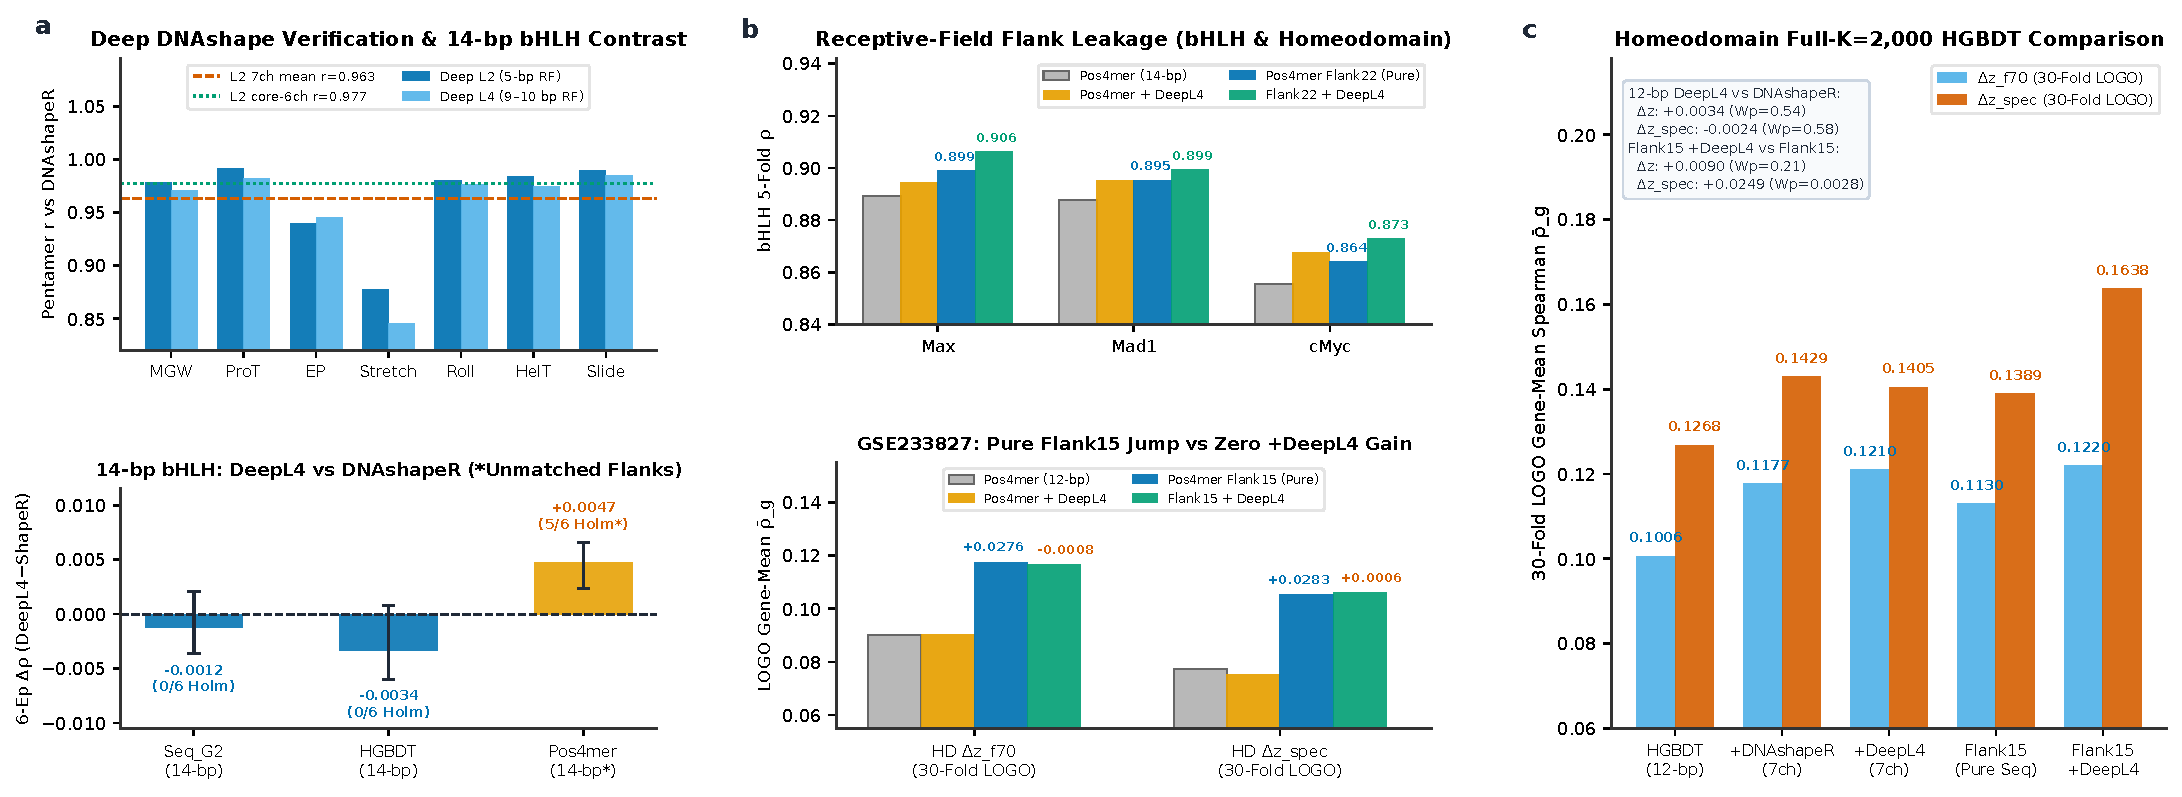
\includegraphics[width=\textwidth]{figures/fig7_deep_dnashape_comparison.pdf}
  \caption{\textbf{Context-extended \emph{Deep DNAshape} comparative benchmark and receptive-field flank leakage across bHLH (\texttt{GSE59845}) and homeodomain (\texttt{GSE233827}).} (\textbf{a}) Top: Layer~2 (5-bp RF) and Layer~4 (9--10~bp RF) pentamer correlation with \texttt{DNAshapeR} across 7 RC-even channels (L2 mean $r = 0.963$ 7ch / $0.977$ core-6ch). Bottom: 6-endpoint mean $\Delta\rho$ (\texttt{DeepL4} $-$ \texttt{DNAshapeR}) on 14-bp bHLH baselines (\texttt{Seq\_G2} $-0.0012$, \texttt{HGBDT} $-0.0034$, 0/6 Holm-sig). (\textbf{b}) Receptive-field flank leakage exposed by flank-matched pure-sequence controls (\texttt{Pos4mer\_Flank22} on bHLH single TFs; \texttt{Pos4mer\_Flank15} jumping $+0.0276/+0.0283$ on \texttt{GSE233827} vs.\ $-0.0008/+0.0006$ for \texttt{+DeepL4}). (\textbf{c}) Homeodomain full-$K=2{,}000$ \texttt{HGBDT} 30-fold LOGO comparison.}
  \label{fig:fig7}
\end{figure}

Evaluating official default Layer~4 (\texttt{DeepL4}, 9--10~bp receptive field, $\pm 4\text{--}5$~bp flanks) against static \texttt{DNAshapeR} and strictly flank-matched pure-sequence controls (\texttt{Flank22} on bHLH; \texttt{Flank15} \texttt{[F-5..F+2]} on homeodomain) revealed both flank leakage and honest residual boundaries (Fig.~\ref{fig:fig7}a--c). On 14-bp bHLH \texttt{GSE59845} (6 endpoints, 5-fold central-10mer \texttt{GroupKFold}), \texttt{DeepL4} failed to outperform \texttt{DNAshapeR} on \texttt{Seq\_G2} ($-0.00122$, 0/6 Holm-sig) or \texttt{HGBDT} ($-0.00336$, 0/6 Holm-sig). While naive 14-bp \texttt{Pos4mer + DeepL4} added $+0.00734$ (6/6 Holm-sig; $+0.00472$ vs.\ \texttt{DNAshapeR}), upgrading pure sequence to flank-matched \texttt{Pos4mer\_Flank22} exposed outer-flank receptive-field leakage on single-TF affinity (\texttt{Max}: $0.8991$ vs.\ $0.8945$; \texttt{Mad1}: $0.8954$ vs.\ $0.8953$; \texttt{cMyc}: $0.8641$ vs.\ $0.8674$). Conditioned strictly on \texttt{Pos4mer\_Flank22}, \texttt{+DeepL4} retained a modest mean gain of $+0.00503$ (4/6 two-sided Holm-sig; $-0.0021$ on \texttt{Mad1$-$Max}), and $+0.01166$ on \texttt{HGBDT\_Flank22} (5/6 two-sided Holm-sig). On homeodomain \texttt{GSE233827} (30-fold LOGO, 92 mutants), \texttt{DeepL4} yielded zero linear gain on either 12-bp or 15-bp pure sequence: expanding pure sequence to \texttt{Pos4mer\_Flank15} jumped by $+0.0276$ ($\Delta z_{f70}$: $0.0900 \to 0.1176$, $W_p = 0.080$) and $+0.0283$ ($\Delta z_{\mathrm{spec}}$: $0.0772 \to 0.1055$, $W_p = 1.37\times 10^{-4}$, 24/30 genes positive), whereas adding \texttt{DeepL4} on top gave $-0.0008$ ($W_p = 0.79$) and $+0.0006$ ($W_p = 0.95$). On full-$K=2{,}000$ \texttt{HGBDT}, 12-bp \texttt{+DeepL4} was statistically indistinguishable from \texttt{DNAshapeR} on $\Delta z_{f70}$ ($+0.0034$, $W_p = 0.54$) and slightly below it on $\Delta z_{\mathrm{spec}}$ ($-0.0024$, $W_p = 0.58$; pure \texttt{HGBDT\_Flank15} reached mutant-mean $0.1402$ vs.\ $0.1328$ for \texttt{12-bp + DeepL4}), while \texttt{HGBDT\_Flank15 + DeepL4} added non-significant $+0.0090$ ($W_p = 0.21$) on $\Delta z_{f70}$ and $+0.0249$ ($0.1389 \to 0.1638$, $W_p = 0.0028$, 22/30 genes; N-arm 11/12 $W_p = 0.0068$; \texttt{specificity\_yes} $W_p = 0.105$) on $\Delta z_{\mathrm{spec}}$, reflecting the continuous tree-splitting proxy geometry analyzed in Section~2.5.

\subsection{Algebraic Complexity-Matching Boundary and Recommended Four-Step Protocol}
Our experiments establish a general complexity-matching theorem for surrogate lookup-table inference: a valid surrogate null must preserve the target table's functional complexity strictly above the conditioning sequence space $\mathcal{F}_{\mathrm{seq}}$. Because \texttt{Sparse4mer} builds residuals solely from 4-mer indicators, conditioning on \texttt{Seq\_Pos4mer} projects out \texttt{Sparse4mer}'s residual degrees of freedom while leaving \texttt{F\_true}'s 5-mer ($r = 5$) variance untouched; thus \texttt{Sparse4mer} is valid on \texttt{Seq\_G2} and tree models, whereas \texttt{ShiftGC\_ExactCRT} is required on \texttt{Seq\_Pos4mer}. Synthesizing all six cohorts (Fig.~\ref{fig:fig6}a--b), apparent ``+Shape'' gains systematically decay toward zero under strong sequence controls and matched surrogates, motivating our four-step calibrated attribution protocol incorporating receptive-field flank matching and Holm--Bonferroni control~\cite{holm1979scand,benjamini1995jrssb}.

\begin{figure}[htbp]
  \centering
  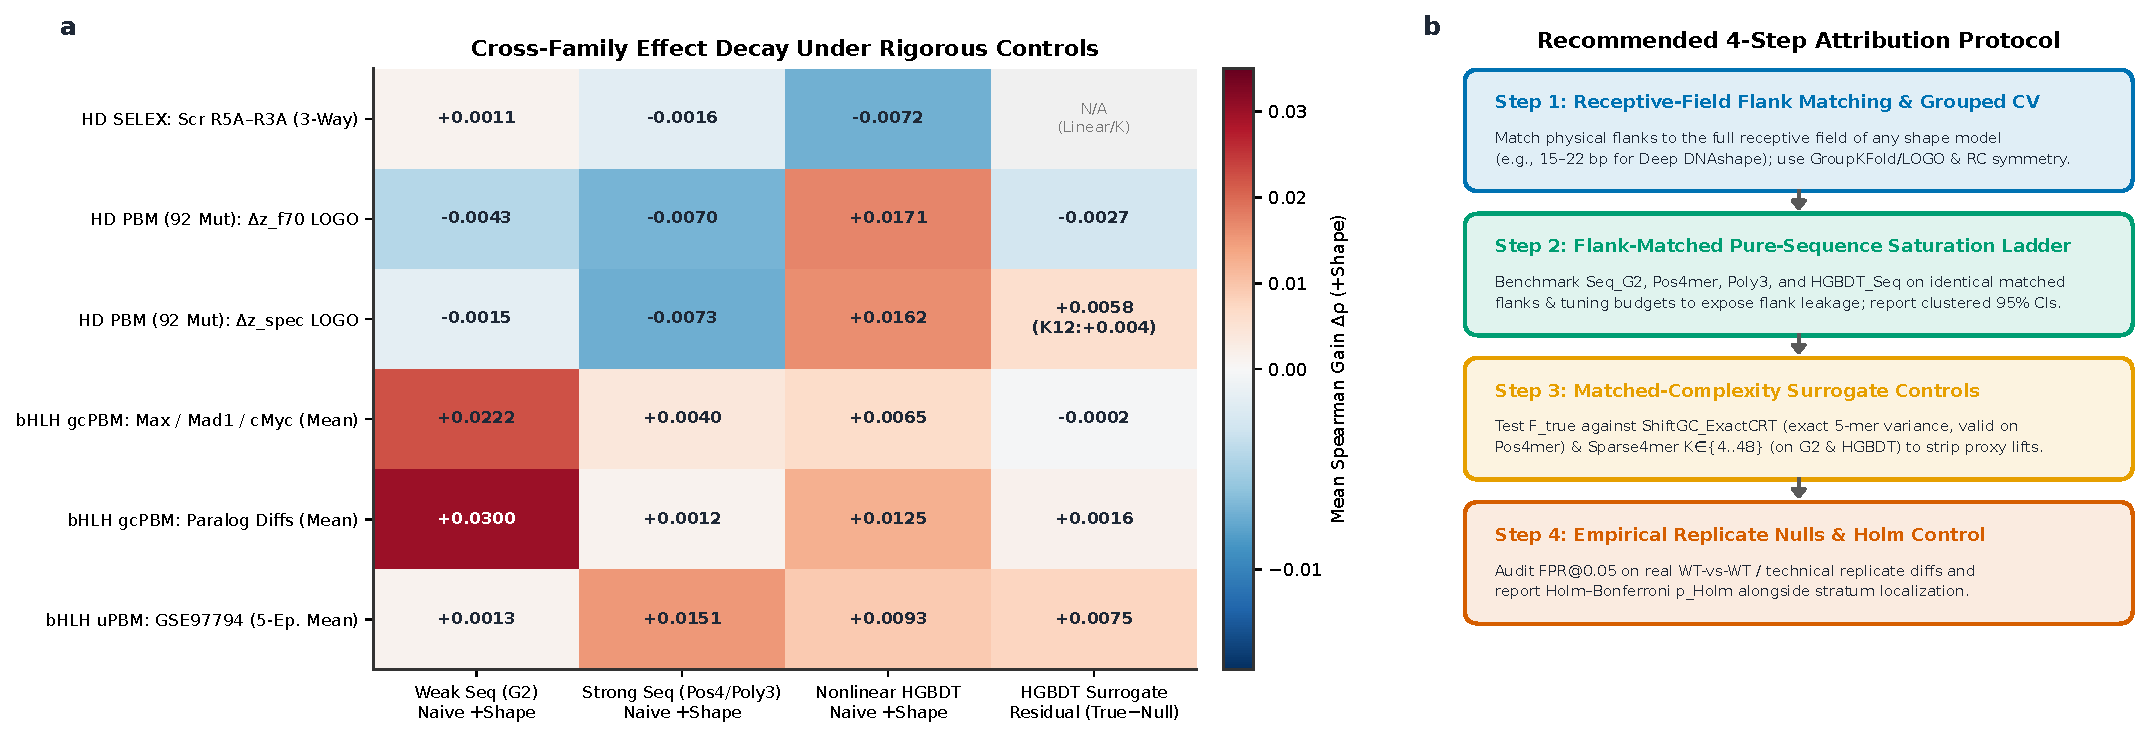
\includegraphics[width=\textwidth]{figures/fig6_unified_attribution_framework.pdf}
  \caption{\textbf{Cross-family effect decay under rigorous controls and recommended four-step attribution protocol.} (\textbf{a}) Unified synthesis heatmap (diverging colormap centered at $0.000$) of mean Spearman gain $\Delta\rho$ across all six benchmark cohorts (updated with full-$K=2{,}000$ $B=19$ residual on $\Delta z_{\mathrm{spec}}$). (\textbf{b}) Four-step calibrated biophysical attribution workflow incorporating receptive-field flank matching.}
  \label{fig:fig6}
\end{figure}

\section{Discussion}
While biophysical experiments conclusively establish that TFs sense three-dimensional DNA geometry~\cite{rohs2009nature,joshi2007cell,abe2015cell,afek2020nature}, our multi-family benchmark demonstrates that sequence-indexed DNA shape predictors---both static pentamer DNAshapeR tables and context-extended \emph{Deep DNAshape}~\cite{chiu2016bioinf,li2017nar,li2024natcomm,li2024nar}---rarely confer reproducible linear out-of-distribution generalization beyond receptive-field-matched pure-sequence representations or complexity-matched random lookup tables. In linear models, pentamer tables act as unmodeled 4/5-mer sequence expansions; in gradient-boosted trees, arbitrary continuous pentamer tables provide smooth split-compression axes~\cite{strobl2007bmc,ke2017lightgbm} reproducing 100\% of bHLH tree lifts (11/11 gcPBM/uPBM endpoints) and 64\%--74\% of the full-$K=2{,}000$ homeodomain $\Delta z_{\mathrm{spec}}$ lift under formal $\alpha = 0.05$ power (Exp~1b $B=19$, 0/6 Holm strata significant, N-arm $p = 0.350\text{--}0.500$); and in context-extended neural predictors, mismatched core windows induce receptive-field flank leakage that collapses once pure-sequence flanks match the predictor's 15--22~bp receptive field.

Our scope boundaries are explicit: modest flank-matched residuals persist for \emph{Deep DNAshape} on bHLH \texttt{Pos4mer\_Flank22} ($+0.0050$, 4/6 Holm-sig) and nonlinear \texttt{HGBDT\_Flank15/22} ($+0.0249$ on homeodomain $\Delta z_{\mathrm{spec}}$; $+0.0117$ on bHLH), warranting future context-extended neural surrogate generators, while 3D protein--DNA geometric neural networks (\emph{DeepPBS}~\cite{mitra2024natmeth}) and all-atom molecular dynamics model conformational remodeling outside sequence-only predictors. Additionally, \texttt{GSE233827} is a matched head-to-head benchmark rather than independent external validation of \emph{FamilyCode}~\cite{liu2025nar}, and \texttt{GSE233827}'s 84 independent multi-chamber bipartitions provide stronger null calibration than \texttt{GSE59845}'s rank-6 within-array pairs.

\section{Methods}

\subsection{Datasets, Alignment, and Homology-Grouped Cross-Validation}
All benchmarks ran strictly on CPU with zero network calls in core modeling modules. Exd--Hox SELEX-seq (\texttt{GSE65073}~\cite{slattery2011cell,abe2015cell}) and 92-mutant human homeodomain PBM (\texttt{GSE233827}~\cite{kock2024natcomm}) cohorts used exact physical flanks (zero \texttt{N}-padding for 12-bp cores) and homology-grouped or 30-fold LOGO cross-validation. For bHLH, our \textbf{Aligned E-box 14-bp Core Grouping} module (\texttt{align\_ebox\_14bp\_cores}) aligns 8,000 paired \texttt{GSE59845} probes~\cite{gordan2013cellrep} strictly by sequence to 7,289 unique RC-canonical 14-bp cores across 1,238 central-10mer homology groups, while our \textbf{Orthogonal uPBM Paralog Differential Benchmark} (\texttt{parse\_gse97794\_upbm\_cohorts}) extracts and globally log-$z$-normalizes 3,620 aligned E-box cores across 2,043 homology groups from \texttt{GSE97794}~\cite{shen2018cels}.

\subsection{Sequence, Kernel, Tree, Surrogate, and Deep DNAshape Modules}
Our \textbf{RC-Symmetrized Positional 4-mer \& G2 Features} module (\texttt{build\_rc\_sym\_ebox\_features}) builds strictly RC-invariant (\texttt{err} $= 0.00$) mononucleotide, dinucleotide, 11-slot positional 4-mer, and 1-bp pentamer tensors solved via two-penalty Ridge regression~\cite{hoerl1970tech} (primary bHLH models use 3 inner folds with $\lambda_{\mathrm{mod}} \in [0.1, 10^4]$; fast null-bank solvers use 2 inner folds with $\lambda_{\mathrm{mod}} \in [0.1, 10^3]$ identically across \texttt{F\_true} and all 1,592 null tables, with outer-train-fold standardization and zero outer-test leakage). Nonlinear baselines comprise our \textbf{Degree-3 Polynomial Kernel Ridge} solver (\texttt{fit\_predict\_poly3\_kernel\_ridge}, exact Woodbury parity $\le 1.82\times 10^{-15}$) and \texttt{HistGradientBoostingRegressor}~\cite{friedman2001aos,ke2017lightgbm,pedregosa2011jmlr}.

Our \textbf{Multi-Sparsity Sparse4mer \& ExactCRT Null Calibration} generator (\texttt{generate\_multisparsity\_null\_bank}) contrasts real 7-channel DNAshapeR tables against \texttt{Naive\_RC\_Perm}, \emph{Shapelizer}~\cite{rube2018msb}, \texttt{ShiftGC\_ExactCRT\_WS\_G2}~\cite{candes2018jrssb,berrett2020jrssb}, and \texttt{Sparse4mer} ($K \in \{4, 8, 12, 24, 48\}$) using exact finite-sample $p_{\mathrm{mc}} = (1 + k)/(B + 1)$~\cite{phipson2010sagmb}. Nonlinear tree attribution uses our \textbf{High-Resolution HGBDT Matched Surrogate Evaluator} (\texttt{evaluate\_hgbdt\_surrogate\_table\_logo}) with locked deterministic hyperparameters across \texttt{Seq\_Only}, \texttt{F\_true}, and all surrogates ($B = 49$ in Exp~1a and bHLH; $B = 9$ bridge on Exp~1b $\Delta z_{f70}$ and formally powered $B = 19$, $p_{\min} = 0.050$ on Exp~1b $\Delta z_{\mathrm{spec}}$). Our \textbf{Context-Extended Deep DNAshape Benchmark} (\texttt{run\_benchmark\_a\_bhlh}, \texttt{run\_benchmark\_b\_gse233827}, \texttt{src/deep\_dnashape\_bench.py}) loads official pre-trained Rohs-Lab TensorFlow~2 checkpoints~\cite{li2024natcomm,li2024nar} offline on CPU via pure-Python SSTable parsing and PyTorch message-passing GRU inference (exact RC equivariance $\max |\mathrm{err}| = 0.00$), benchmarking Layer~2/Layer~4 against static \texttt{DNAshapeR} and strictly flank-matched pure-sequence controls (\texttt{Flank22} on \texttt{GSE59845}; \texttt{Flank15} on \texttt{GSE233827}). Empirical negative controls rely on \texttt{GSE233827} multi-chamber WT-vs-WT splits and our \textbf{Within-Array Technical Replicate Negative Controls} parser (\texttt{parse\_gse59845\_replicate\_cohorts}), paired with cluster bootstrapping~\cite{efron1993boot,cameron2008restat} and Holm--Bonferroni control~\cite{holm1979scand}. Strictly inductive deployment is verified via our \textbf{Inductive Pos4mer Ridge Predictor} (\texttt{run\_inductive\_pos4mer\_ridge}, \texttt{src/predict.py}; \texttt{cMyc$-$Max} Fold-0 $R^2 = 0.6362$, Spearman $= 0.7644$, row-permutation invariance $\le 10^{-12}$).

\bibliographystyle{unsrtnat}
\bibliography{references}
\end{document}
